\section{TCP Vegas}

\subsection{Congestion avoidance}

Reaction to congestion episode, not to packets loss

Modifications:

\begin{itemize}
  \item Modified Congestion Avoidance
  \item Aggressive Retransmission
  \item Aggressive Window Adaptation
  \item Modified SS phase
\end{itemize}

Some definitions:

\begin{itemize}
  \item \textbf{Throughput}: speed of transmission
  \item \textbf{Goodput}: speed of reception
\end{itemize}

Comparing expected and actual throughput:

\begin{itemize}
  \item \textbf{Expected throughput}: $\frac{window\_size}{RTT}$
  \item \textbf{Actual throughput}: $\frac{actual\_transmitted\_amount}{RTT}$
\end{itemize}

Monitor transmission rate: \\

$\diamond$ If $expected - \alpha < actual < expected$:
Queues decreasing $\rightarrow$ increase rate \\

$\diamond$ If $expected - \alpha < actual < expected - \beta$:
Don’t do anything \\

$\diamond$ If $actual < expected - \beta$:
Queues increasing $\rightarrow$ decrease rate before packet drop (maybe there
is a congestion in network or maybe the connection is shared among other
services) \\

Thresholds of $\alpha (= \frac{1 pkts}{RTT})$ and $\beta (= \frac{3 pkts}{RTT})$ correspond to how many packets 
Vegas is willing to have in queues.

\begin{figure}[H]
  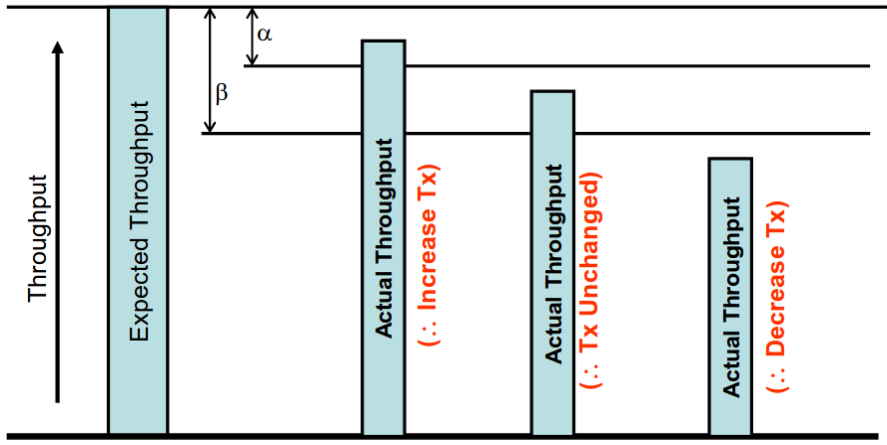
\includegraphics[scale=0.35]{CAVegas}
  \caption{Vegas - Modified Congestion Avoidance}
\end{figure}




